\section{Operation of the Vending Circuit}

\subsection{Initialization}
\begin{enumerate}
\item The states of the flip flops should reflect the amount of money that has been put into the machine.
\end{enumerate}

\subsection{How to Vend an Item}
\begin{enumerate}
\item We need to select the subtract function on the ALU instead of the add function. This is accomplished by switch number 7 on the board and a quad 2-1 mux (74LS157) that outputs the combinations of selector bits that tell the ALU to either add or subtract. You can call it the selector bit selector if you would like. 
\begin{figure}[H]
\centering
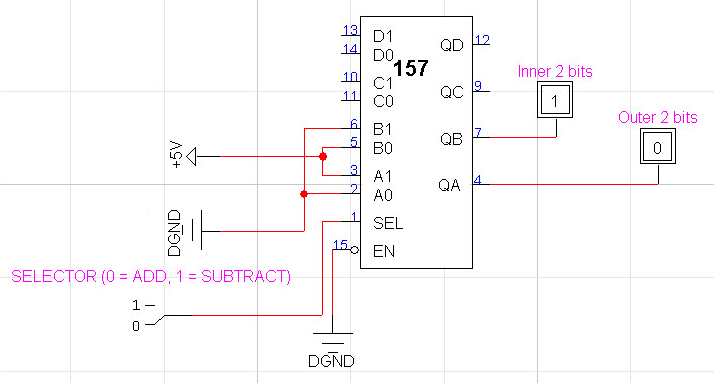
\includegraphics[width=12cm]{selector-bit-selector} \\
%\vspace{1em} \hspace{1em}
\caption{The selector bit selector takes advantage of the fact that in the patterns for selecting the ADD and SUBTRACT functions on the ALU, $S_0 = S_4$ and $S_2 = S_3$}. Because of this, we can use only two of the four outputs to select addition (0110) and subtraction (1001). 
\label{selector-bit-selector}
\end{figure}

\item Vending should only happen if the price of the item is less than or equal to the amount of money in the machine. We check this by subtracting the price of the item from the dollars in machine and checking the seventh bit of the output. Since we only work with 6 bit numbers, any non-zero value of the seventh bit will mean that an overflow occurred and that there is not enough money in the machine to vend the item. This check, however, should only occur if we are performing subtraction and since we use the same circuit components to do addition and subtraction we need some extra logic to make it work. The circuit shown below is used to determine when a clock pulse should be allowed to reach the flip flops.
\begin{figure}[H]
\centering
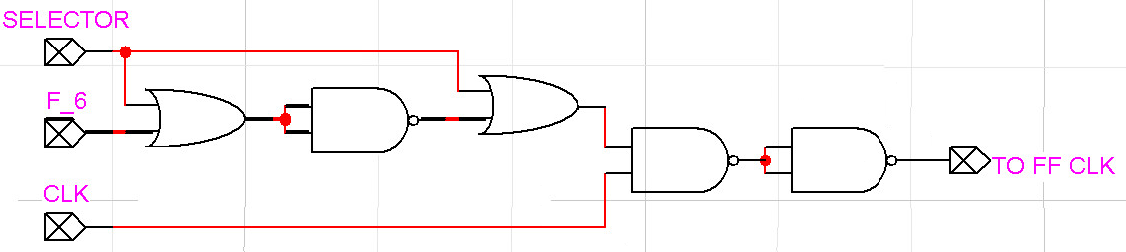
\includegraphics[width=12cm]{clock-enable} \\
%\vspace{1em} \hspace{1em}
\caption{This set of gates was chosen because there were three free NAND gates on the board as well as several OR gates. This is definitely not the simplest way to implement this logic, however. A more simplified version that is easier to follow is below in Figure \ref{clock-enable-simplified}.}
\label{clock-enable}
\end{figure}
\begin{figure}[H]
\centering
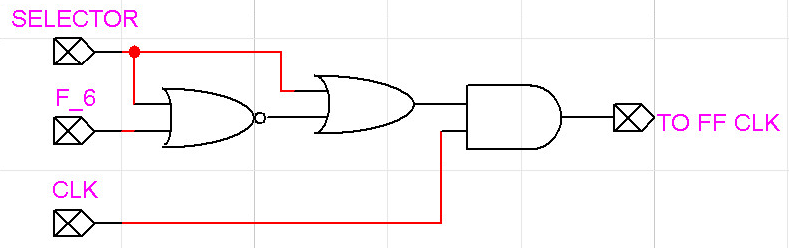
\includegraphics[width=10cm]{simplified-clock-enable} \\
%\vspace{1em} \hspace{1em}
\caption{The functionality of this circuit is equivalent to the one above in Figure \ref{clock-enable}, but it would have required adding a NOR chip and an AND chip to the board.}
\label{clock-enable-simplified}
\end{figure}
\end{enumerate}
